\begin{figure}[H]
\centering
\includegraphics[page=4,width=0.3\textwidth]{\FCNCFigures/xTFW/showFake/NOMINAL/reg2mtau1b2jos_vetobtagwp70_highmet/BDTG_test.pdf}
\includegraphics[page=5,width=0.3\textwidth]{\FCNCFigures/xTFW/showFake/NOMINAL/reg2mtau1b2jos_vetobtagwp70_highmet/BDTG_test.pdf}
\includegraphics[width=0.3\textwidth]{\FCNCFigures/xTFW/BDT/roc_reg2mtau1b2jos.pdf}\\
\includegraphics[page=4,width=0.3\textwidth]{\FCNCFigures/xTFW/showFake/NOMINAL/reg2mtau1b3jos_vetobtagwp70_highmet/BDTG_test.pdf}
\includegraphics[page=5,width=0.3\textwidth]{\FCNCFigures/xTFW/showFake/NOMINAL/reg2mtau1b3jos_vetobtagwp70_highmet/BDTG_test.pdf}
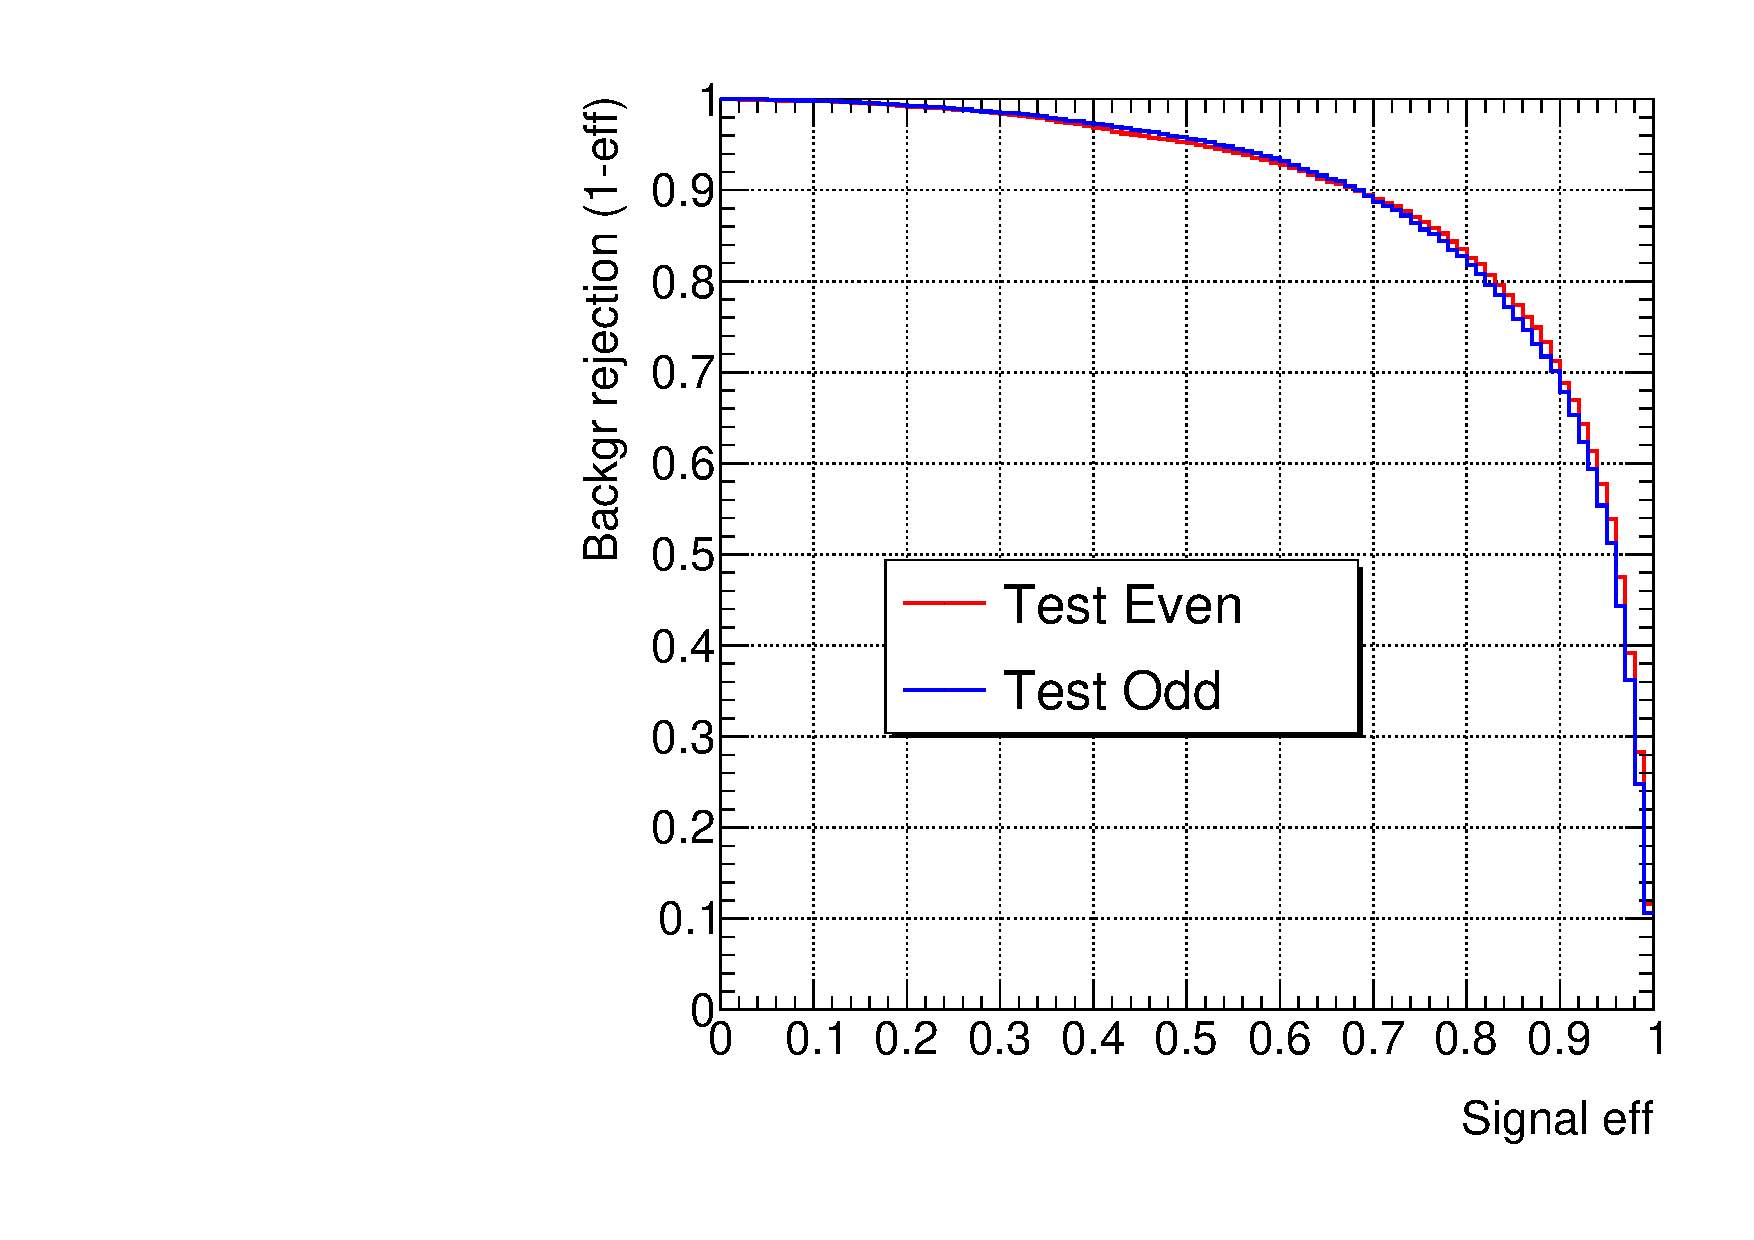
\includegraphics[width=0.3\textwidth]{\FCNCFigures/xTFW/BDT/roc_reg2mtau1b3jos.pdf}\\
\includegraphics[page=4,width=0.3\textwidth]{\FCNCFigures/tthML/showFake/faketau/postfit/NOMINAL/reg1l1tau1b2j_os_vetobtagwp70_highmet/BDTG_test.pdf}
\includegraphics[page=5,width=0.3\textwidth]{\FCNCFigures/tthML/showFake/faketau/postfit/NOMINAL/reg1l1tau1b2j_os_vetobtagwp70_highmet/BDTG_test.pdf}
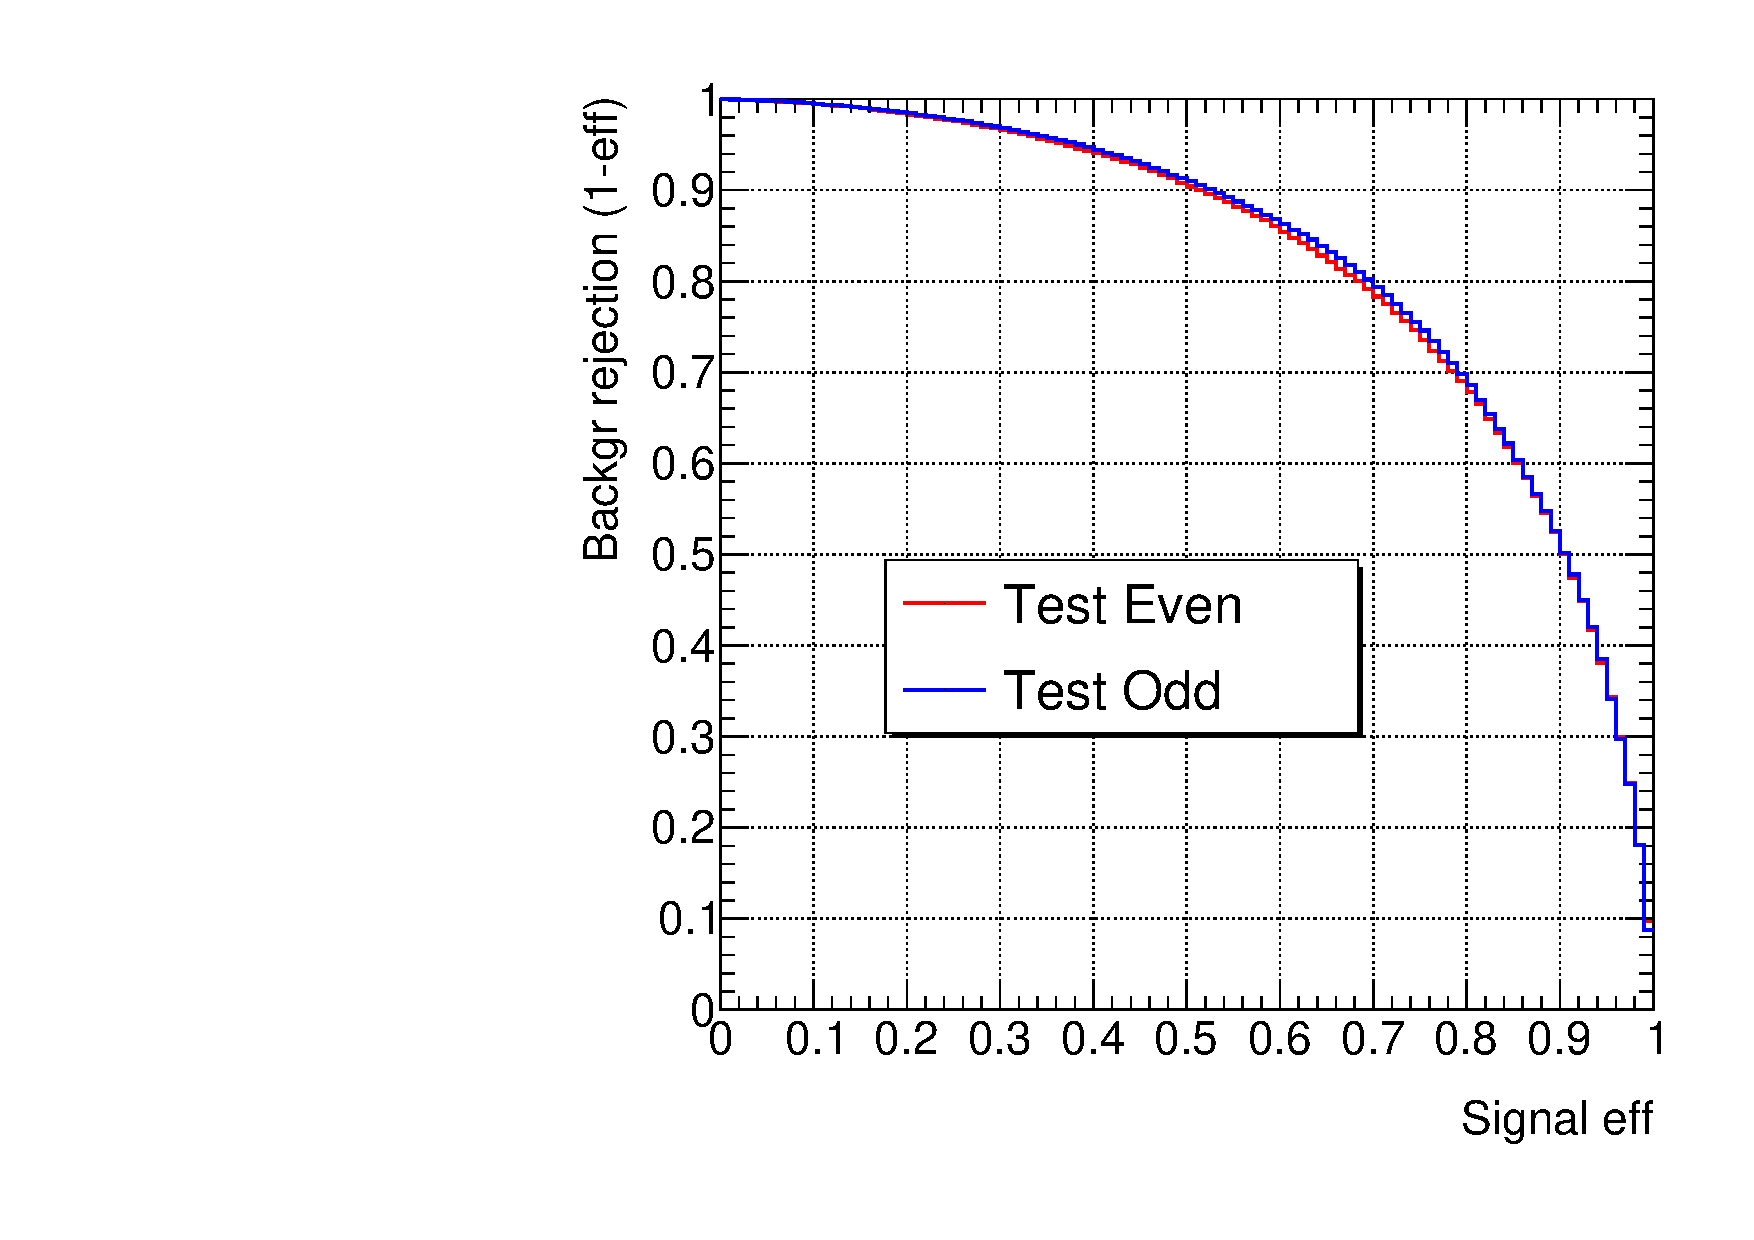
\includegraphics[width=0.3\textwidth]{\FCNCFigures/tthML/BDT/roc_reg1l1tau1b2j_os.pdf}\\
\includegraphics[page=4,width=0.3\textwidth]{\FCNCFigures/tthML/showFake/faketau/postfit/NOMINAL/reg1l1tau1b3j_os_vetobtagwp70_highmet/BDTG_test.pdf}
\includegraphics[page=5,width=0.3\textwidth]{\FCNCFigures/tthML/showFake/faketau/postfit/NOMINAL/reg1l1tau1b3j_os_vetobtagwp70_highmet/BDTG_test.pdf}
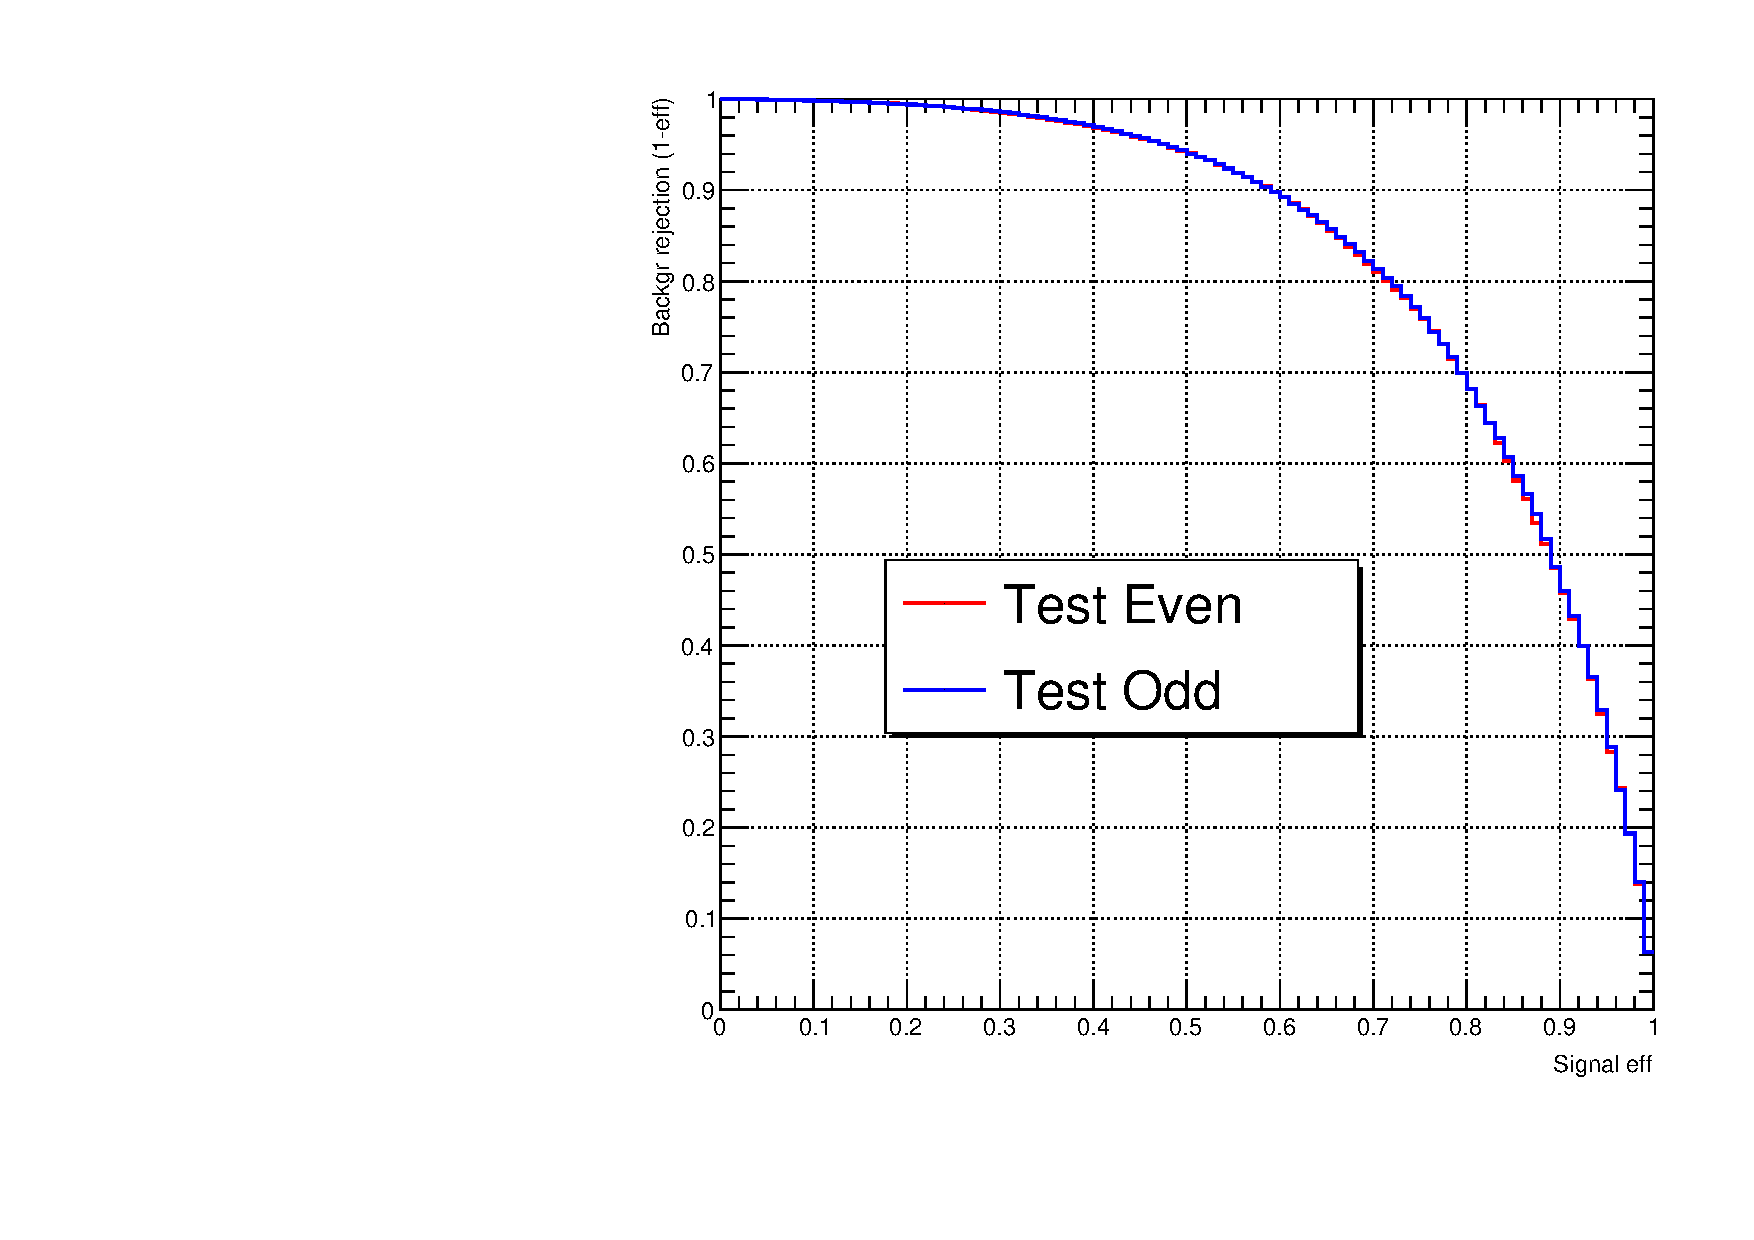
\includegraphics[width=0.3\textwidth]{\FCNCFigures/tthML/BDT/roc_reg1l1tau1b3j_os.pdf}\\
\caption{强子道的两个信号区与两个$\tlhad$信号区中,使用BDT交叉测试所得的BDT分数分布,左图为tuH FCNC耦合的衰变模式与本底的比较,中间的图为tuH FCNC耦合的产生模式与本底的比较,右图为交叉验证的ROC曲线比较。}
\label{fig:overtrain_lephad}
\end{figure}
\begin{figure}[H]
\centering
\includegraphics[page=4,width=0.3\textwidth]{\FCNCFigures/tthML/showFake/faketau/postfit/NOMINAL/reg1l2tau1bnj_os/BDTG_test.pdf}
\includegraphics[page=5,width=0.3\textwidth]{\FCNCFigures/tthML/showFake/faketau/postfit/NOMINAL/reg1l2tau1bnj_os/BDTG_test.pdf}
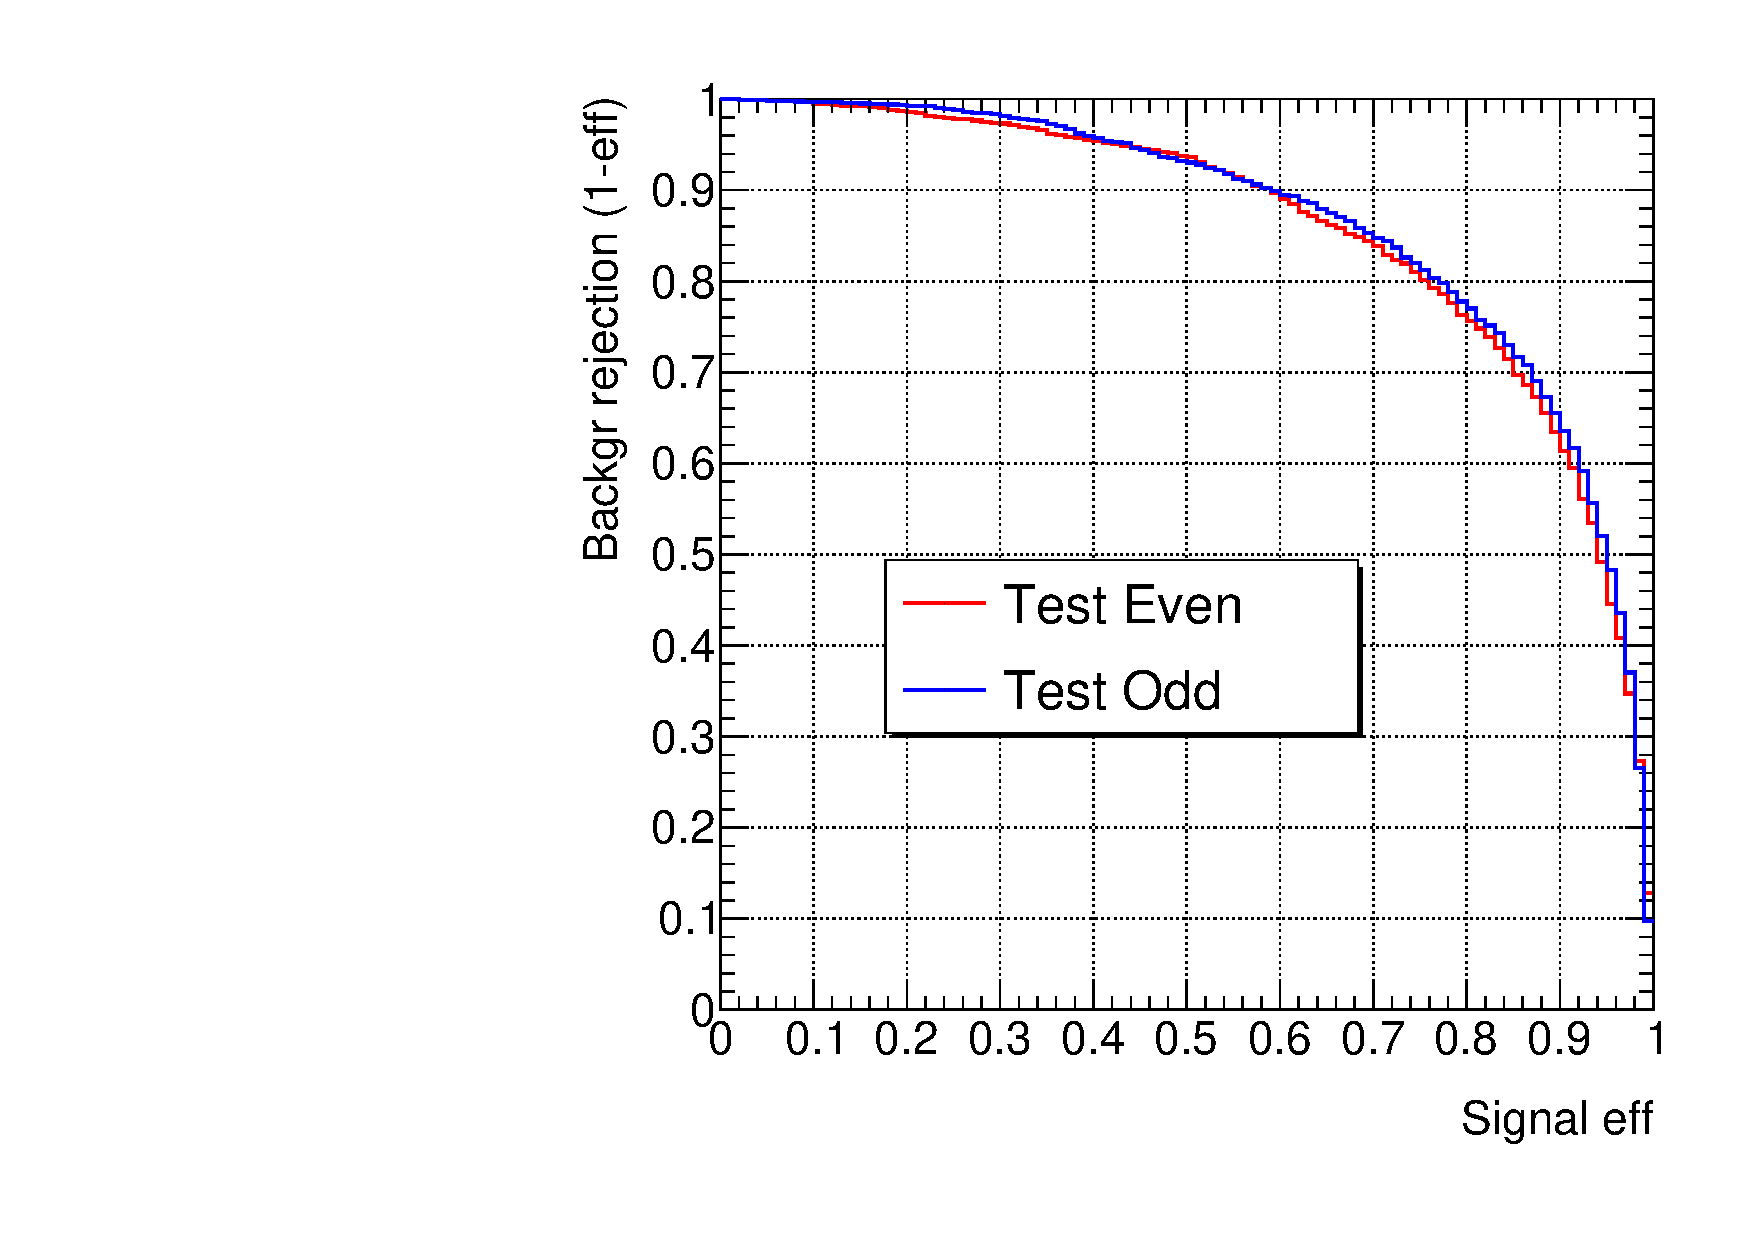
\includegraphics[width=0.3\textwidth]{\FCNCFigures/tthML/BDT/roc_reg1l2tau1bnj_os.pdf}\\

\includegraphics[page=4,width=0.3\textwidth]{\FCNCFigures/tthML/showFake/faketau/postfit/NOMINAL/reg1l1tau1b1j_ss_vetobtagwp70_highmet/BDTG_test.pdf}
\includegraphics[page=5,width=0.3\textwidth]{\FCNCFigures/tthML/showFake/faketau/postfit/NOMINAL/reg1l1tau1b1j_ss_vetobtagwp70_highmet/BDTG_test.pdf}
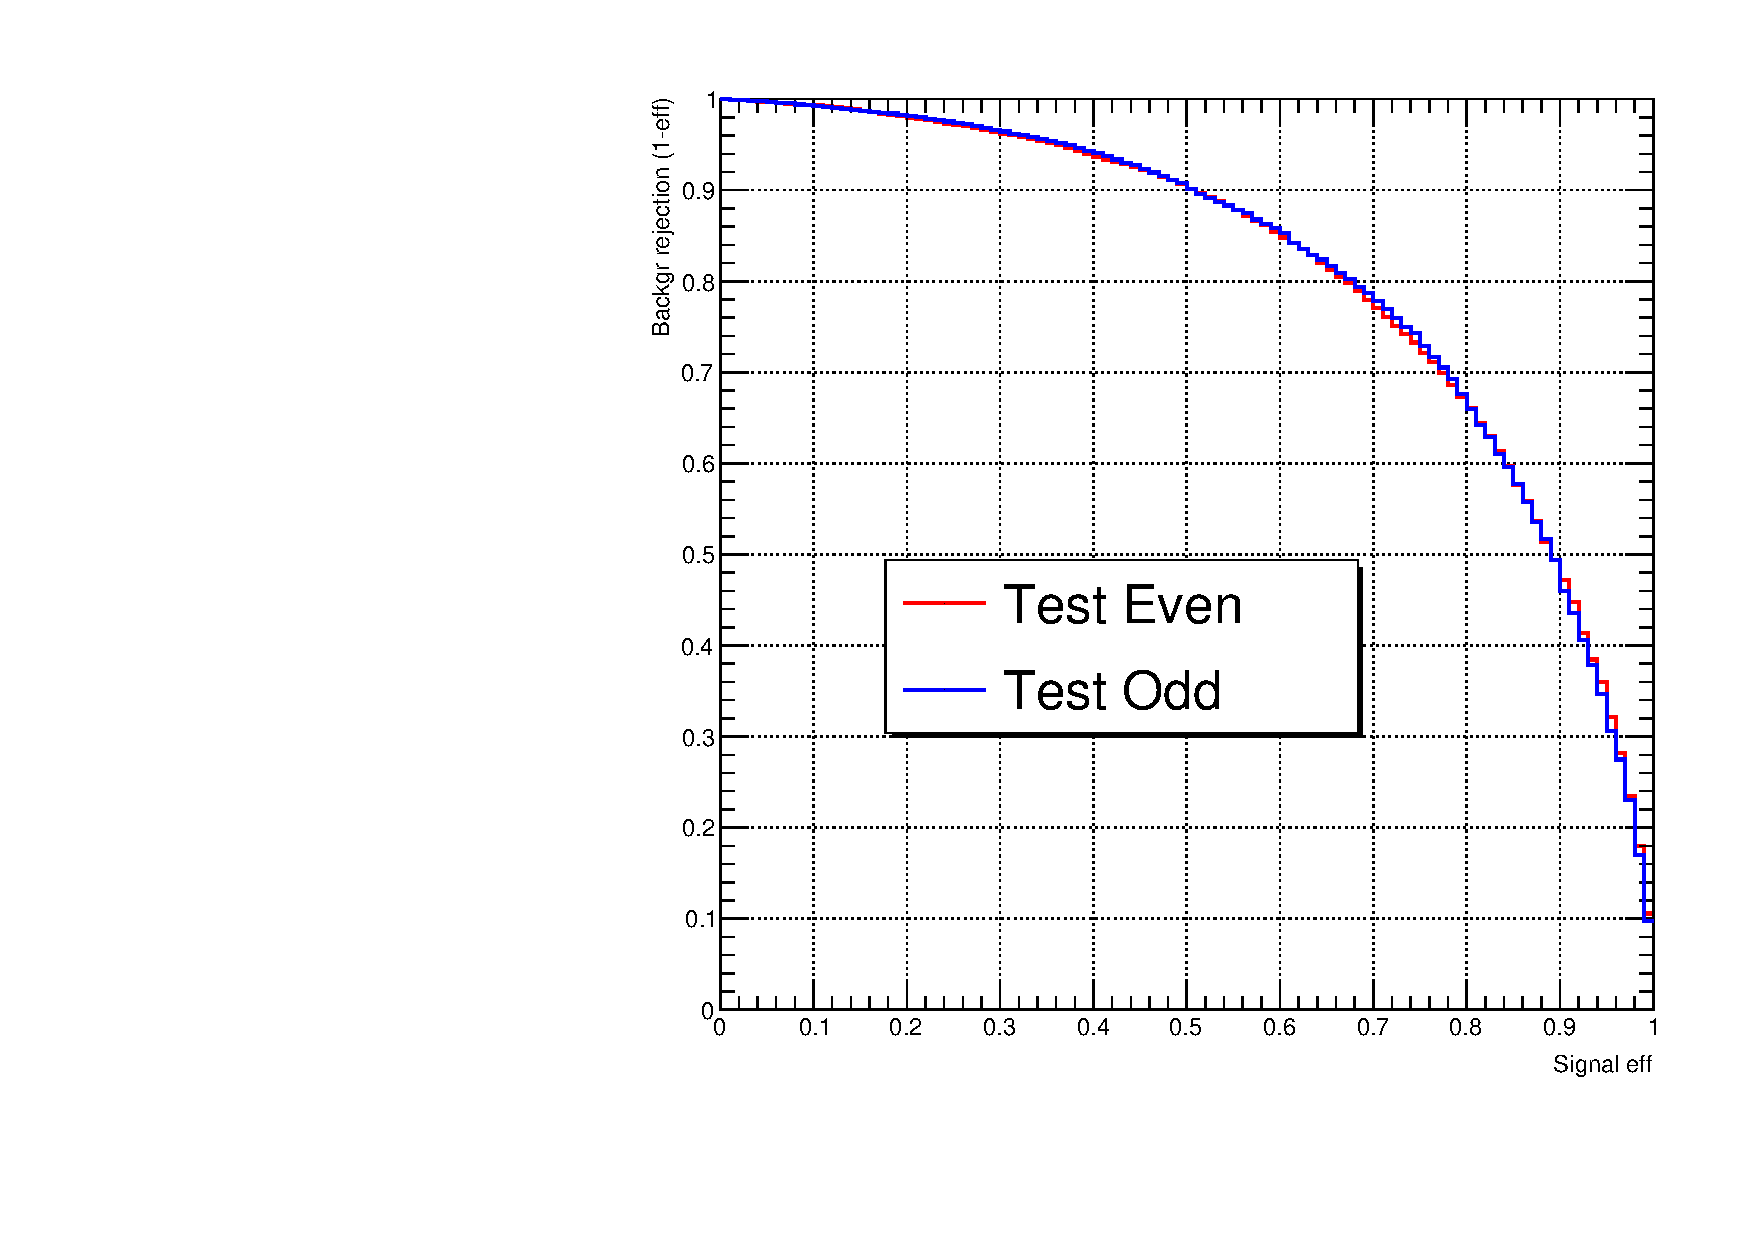
\includegraphics[width=0.3\textwidth]{\FCNCFigures/tthML/BDT/roc_reg1l1tau1b1j_ss.pdf}\\

\includegraphics[page=4,width=0.3\textwidth]{\FCNCFigures/tthML/showFake/faketau/postfit/NOMINAL/reg1l1tau1b2j_ss_vetobtagwp70_highmet/BDTG_test.pdf}
\includegraphics[page=5,width=0.3\textwidth]{\FCNCFigures/tthML/showFake/faketau/postfit/NOMINAL/reg1l1tau1b2j_ss_vetobtagwp70_highmet/BDTG_test.pdf}
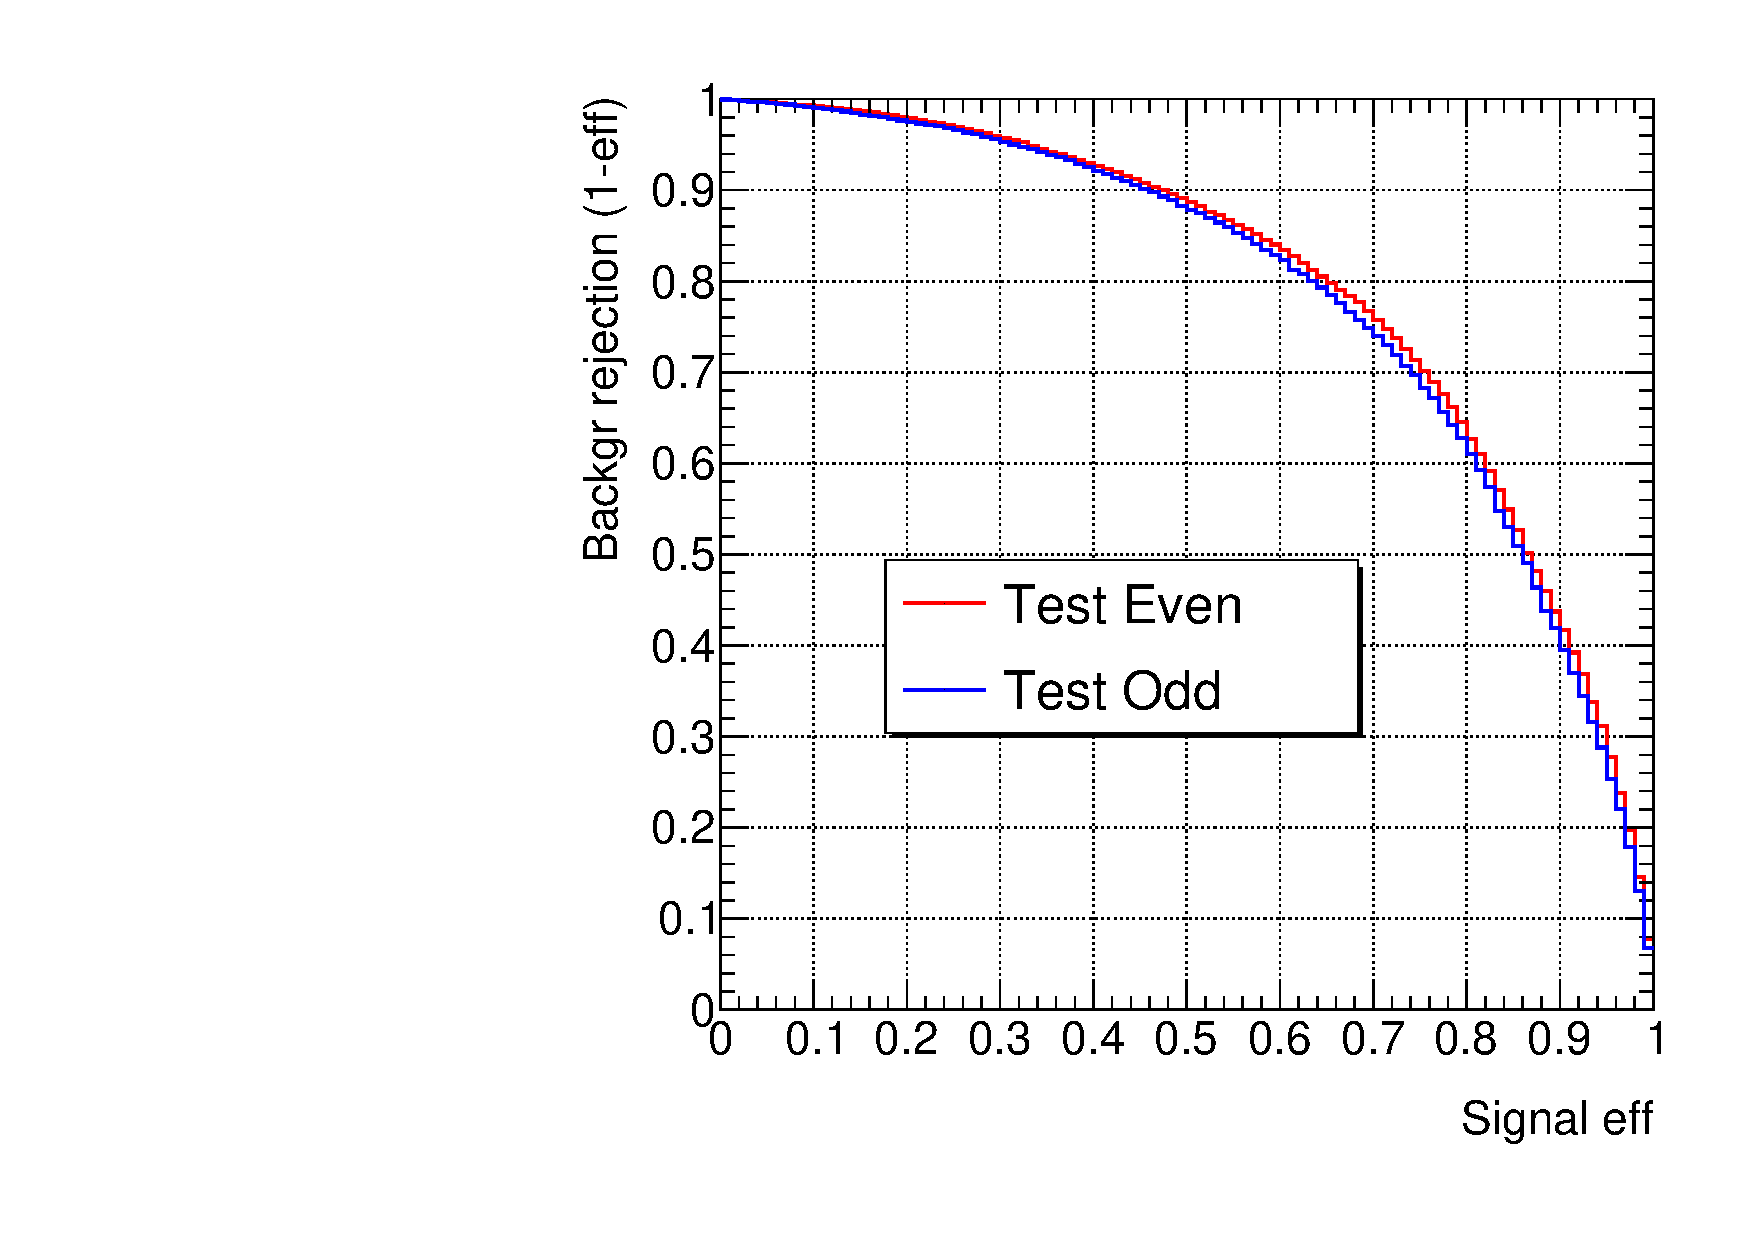
\includegraphics[width=0.3\textwidth]{\FCNCFigures/tthML/BDT/roc_reg1l1tau1b2j_ss.pdf}\\

\caption{$l\thadhad$和两个$l\tauhad$信号区使用BDT交叉测试所得的BDT分数分布,左图为tuH FCNC耦合的衰变模式与本底的比较,中间的图为tuH FCNC耦合的产生模式与本底的比较,右图为交叉验证的ROC曲线比较。}
\label{fig:overtrain_hadhad}
\end{figure}
